\documentclass{article}
\usepackage[utf8]{inputenc}

\usepackage{times}
\usepackage{graphicx}
\usepackage{amsmath}
\usepackage{amsfonts}
\usepackage{amssymb}
\usepackage{color, soul}
\usepackage{natbib} 

\renewcommand{\vec}[1]{\boldsymbol{{#1}}} 

\title{The Climate Machine (CLIMA)}
\author{Climate Modeling Alliance}

\begin{document}

\maketitle

\section{Overview}

To achieve a step change in the accuracy and precision of climate simulations and predictions, we are developing CLIMA, an Earth system model (ESM) that learns automatically from diverse data sources. Our goal is to use observational data along with modern computational methods not simply to evaluate and test models, as is current practice, but to systematically reduce model-data mismatches and quantify uncertainties. To accomplish this goal, we will harness, simultaneously and self-consistently, orders-of-magnitude more data than are currently used in model development, exploiting new techniques from data assimilation (DA) and machine learning (ML).

\subsection{Automated Learning From Observations and High-Resolution Simulations}

We will design an ESM platform with subgrid-scale (SGS) process models that learn automatically from two sources of information (for more details and references, see \citet{Schneider17c}, from which several passages of this document are taken):
\begin{enumerate}
    \item \emph{Global observations.} We live in the golden age of Earth observations from space. A suite of satellites is streaming coordinated and nearly simultaneous measurements of variables such as temperature, humidity, clouds, ocean surface currents, and sea ice cover, with global coverage for more than a decade. Space-based measurements of biogeochemical tracers and processes, such as measurements of column-average CO2 concentrations, of ocean biomass, and of photosynthesis in ecosystems, are also available, and so are more detailed observations of the cryosphere. To date, only a minute fraction of the data (mostly large-scale energy fluxes) has been directly used in ESM development (as opposed to ESM evaluation). CLIMA will learn directly from global data, augmented and validated with more detailed local observations where available.
    \item \emph{Local high-resolution simulations.} Some SGS processes in ESMs are in principle computable, only the globally achievable resolution precludes their explicit computation. For example, the turbulent dynamics of clouds can be computed with high fidelity in limited domains in large-eddy simulations (LES) with mesh sizes of meters to tens of meters. Increased computational performance has made LES domain widths of 10--100~km feasible in recent years, while the horizontal mesh size in climate models has shrunk, to the point that the two scales have converged \citep{Schneider17a}. Thus, while global LES that reliably resolve low clouds will not be feasible for decades, it is now possible to nest LES in limited areas of atmosphere models and conduct targeted local high-fidelity simulations of cloud dynamics in them. Local high-resolution simulations of ocean turbulence or sea ice dynamics can be conducted similarly. CLIMA will learn from such nested high-resolution simulations.
\end{enumerate}
Simultaneously exploiting global observations and local high-resolution simulations with new DA/ML tools presents the key opportunity for  progress in Earth system modeling. Replacing the inefficient and sub-optimal manual tuning process and the offline fitting of parameterization schemes to data from few locations, as is currently common, CLIMA will autotune itself and quantify its uncertainties based on statistics of much larger range of available data. It will adapt as new observations come online, and it will generate targeted high-resolution simulations on the fly---akin to targeted observations in weather forecasting \citep{Palmer98a,Lorenz98a}---to reduce and quantify uncertainties where needed to tighten estimates of SGS models of computable processes. This will increase the amount of data to which SGS models are fitted by several orders of magnitude.

\subsection{Optimization Over Aggregate Climate Statistics}

The automated learning from observations and high-resolution simulations in CLIMA will use \emph{statistics accumulated in time} (e.g., over seasons) to:
\begin{enumerate}
\item Minimize model biases, especially biases that are known to correlate with the climate response of models. This amounts to minimizing mismatches between time averages of ESM-simulated quantities and data.
\item Minimize model-data mismatches in higher-order Earth system statistics. This includes covariances such as cloud-cover/surface temperature covariances, or ecosystem carbon uptake/surface temperature covariances, which are known to correlate with the climate response of models (``emergent constraints''). It can also include higher-order statistics involving direct targets for prediction goals, such as rainfall extremes. 
\end{enumerate}
By optimizing how well an ESM simulates climate statistics, our approach directly targets success metrics that are relevant for climate projections. Optimizing over climate statistics ameliorates problems arising from ill-posedness of the inverse problem (underdetermination of SGS models given data), and it  avoids difficulties caused by sensitive dependences on atmospheric initial conditions and small-scale roughness. These difficulties arise when optimizing over snapshots of Earth system states, as in numerical weather prediction. For example, the challenge of simulating when and where clouds occur, with temporal and spatial accuracy (e.g., hours to minutes in time and kilometers to hundred meters in space), has prevented the routine assimilation of space-based radar and lidar observations of clouds in numerical weather predictions \citep{Stephens18a}. But if these same data are aggregated, for example, over seasons, precisely when and where individual clouds occur, and their sensitive dependence on atmospheric initial conditions, become less important. The aggregated cloud statistics vary smoothly in time and space, and minimizing mismatches in them directly targets what matters for climate projections. This is where the key untapped opportunity lies for CLIMA to radically improve upon existing models.

The problem of minimizing model-data mismatches in climate statistics is computationally challenging because accumulating statistics from an ESM is costly: each evaluation of the target statistics requires an ESM simulation at least over a season. But the computational problems are just beginning to be tractable, for example, with the ensemble-based inversion methods we will develop and employ.

\subsection{Computable and Noncomputable Parameters}

Learning from  local high-resolution simulations and observations is aimed at determining two different kinds of parameters in parameterization schemes: \emph{computable} and \emph{non-computable} parameters. (Since parameters and parametric functions of state variables play essentially the same role in our discussion, we simply use the term parameter, with the understanding that this can include parametric functions and even nonparametric functions.) Computable parameters are those that can in principle be inferred from high-resolution simulations alone. They include parameters in radiative transfer schemes, which can be inferred from detailed line-by-line calculations; dynamical parameters in cloud turbulence parameterizations, such as entrainment rates, which can be inferred from LES; or parameters in ocean mixing parameterizations, which can be inferred from high-resolution simulations. Non-computable parameters are parameters that, currently, cannot be inferred from high-resolution simulations, either because computational limitations make it necessary for them to also appear in parameterization schemes in high-resolution simulations, or because the microscopic equations governing the processes in question are unknown. They include parameters in cloud microphysics parameterizations, which are still necessary to include in LES, and many parameters characterizing ecological and biogeochemical processes, whose governing equations are unknown. Cloud microphysics parameters will increasingly become computable through direct numerical simulation, but ecological and biogeochemical parameters will remain non-computable for the foreseeable future. We will denote computable parameters by $\vec{\theta}_c$ and non-computable parameters by $\vec{\theta}_n$. Jointly, they form the parameter vector $\vec{\theta}=(\vec{\theta}_c, \vec{\theta}_n)$.

Both computable and non-computable parameters can, in principle, be learned from observations; the only restrictions to their identifiability come  from the well-posedness of the learning problem and its computational tractability. But only computable parameters can be learned from targeted high-resolution simulations. To be able to learn computable parameters, it is essential to represent non-computable aspects of a parameterization scheme consistently in the high-resolution simulation and in the parameterization scheme that is to learn from the high-resolution simulation. For example, radiative transfer and microphysical processes need to be represented consistently in a high-resolution LES and in a parameterization scheme if the parameterization scheme is to learn computable dynamical parameters such as entrainment rates from the LES. 

\subsection{Fresh Model Architecture}

\begin{figure}
\centerline{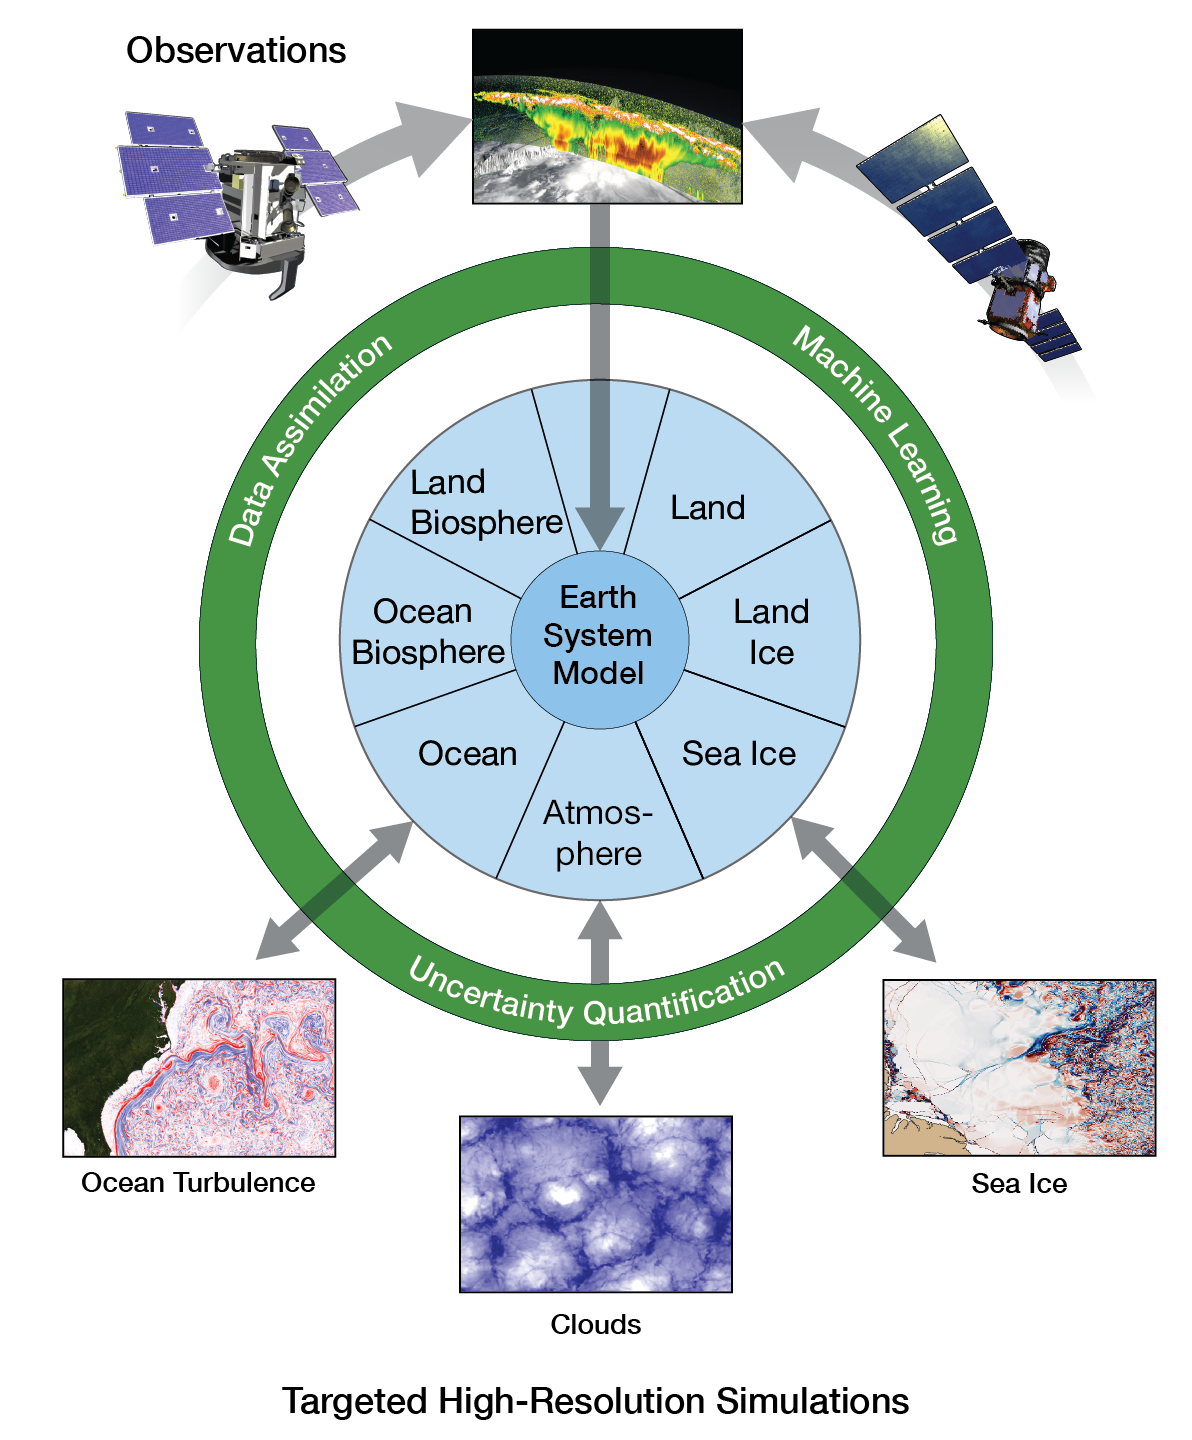
\includegraphics[width=.95\textwidth]{CLIMA-schematic.png}}
\caption{\textbf{Schematic of CLIMA.} Observations of the Earth system (e.g., from space) and output from targeted high-resolution simulations (e.g., of ocean turbulence) are passed through a data assimilation/machine learning (DA/ML) layer, which wraps around an Earth system model (ESM) with its component models. The high-resolution simulations that inform the ESM through the DA/ML layer are spun off from component models such as the atmosphere or ocean models. The DA/ML layer not only optimizes the ESM components but also quantifies uncertainties about model processes.} 
\label{f:CLIMA-schematic}
\end{figure}
CLIMA will have a fresh model architecture (see the schematic in Fig.~\ref{f:CLIMA-schematic}). Current ESM architectures make it difficult to carry out the hundreds to thousands of ESM simulations that are necessary for DA/ML based on climate statistics, and current parameterization schemes are not well suited for DA/ML approaches (e.g., because they contain many correlated parameters).  We will need to design CLIMA to learn efficiently from observations and to run nested high-resolution simulations on the fly, and we will need to replace several existing parameterization schemes by flexible SGS process models that learn effectively from diverse data sources. The SGS process models need to be systematically refine-able as more data become available, and they need to treat subgrid-scale motions (e.g., boundary layer turbulence, shallow convection, deep convection) in a unified manner. Achieving this will be a central focus of our development effort.

To achieve rapid payoffs in terms of reduced uncertainties in climate projections, we will focus the early development on the most uncertain components for which we have already begun development and prototyping of new SGS process models (e.g., for clouds, convection, and turbulence), while initially using other components from existing models. However, we will eventually seek to replace most current parameterization schemes by more flexible SGS process models designed for DA/ML approaches. 

To be fast and run at the highest resolutions feasible, CLIMA will also need to effectively exploit the computing architectures that are currently emerging, including heterogeneous many-core architectures that combine traditional CPUs with hardware accelerators such as graphical processing units (GPUs) or Field Programmable Gate Arrays (FPGAs). Targeted high-resolution simulations nested in a global ESM are ideally suited for running on accelerators, which shine at solving computational problems that can be decomposed into largely independent subtasks that are comparable in computational effort. Many high-resolution simulations---potentially hundreds or thousands---can be run concurrently with the coarse-resolution ESM, avoiding idle computational threads that otherwise limit accelerator efficiency. We may also want to exploit emerging AI accelerator designs, when they are broadly available, in the DA/ML components of the ESM platform.

\section{CLIMA Layers and Goals}

CLIMA consists of several layers (Figs.~\ref{f:CLIMA-schematic} and \ref{f:CLIMA-layers}). Wrapped around what traditionally would be the ESM is a DA/ML layer, whose function it is to connect the ESM with observations and targeted high-resolution simulations, to learn about uncertain SGS processes in the ESM. For example, the DA/ML layer allows the ESM to learn about uncertain SGS models of ocean turbulence through matching simulated statistics of ocean turbulence to those observed by satellite altimeters. Or, the DA/ML layer allows the ESM to learn about uncertain SGS models of clouds, convection, and atmospheric turbulence through matching ESM-simulated statistics of cloud cover and cloud condensate to those obtained from LES spun-off from the atmosphere model.

To design CLIMA to learn from diverse data sources, we will employ the key concepts and pursue the goals described in what follows, moving layerwise from the outside to the computational core.

\subsection{Observations}

\paragraph{Concepts}
\begin{itemize}
    \item Observations are primarily space-based or ground-based observations with large spatial coverage.
    \item Observations can also come from field campaigns, which provide more detailed data that are local in space and time. It remains to be seen whether we want to learn from such local data online in CLIMA, or whether we primarily want to use local data in off-line development and testing of SGS models and to provide prior information for learning in CLIMA.
    \item Observables $\vec{y}$ are linked to state variables $\vec{x}$ of the ESM through a map $\mathcal{H}$ representing an observing system, so that 
    \begin{equation}
    \vec{y}(t)=\mathcal{H}\bigl(\vec{x}(t)\bigr).
    \end{equation}
    The observables $\vec{y}$ might represent surface temperatures, cloud cover, or spectral radiances emanating from the TOA. The map $\mathcal{H}$ projects ESM state variables $\vec{x}$ to observables at the locations and times at which actual observations, denoted by $\vec{\tilde y}$, are available. For complex observing systems (e.g., satellites), the map $\mathcal{H}$ represents an observing system simulator and hence can be complicated. The observations $\vec{\tilde y}$ are independent of the parameters $\vec{\theta}$.
\end{itemize}

\paragraph{Goals}
\begin{itemize}
    \item For the atmosphere, focus first on learning from reanalysis data, including seasonally and spatially varying statistics of variables such as atmospheric temperature and precipitation for the satellite era (from 1980 onward). Reanalyses provide easily accessible and homogenized data, for which the map $\mathcal{H}$ is a simple projection operator. This will allow us to prototype and develop the CLIMA platform more quickly than would be possible if we were to integrate a large set of diverse observational data sources from the outset, which each requires a separate observing system simulator $\mathcal{H}$.
    \item For the ocean, focus first on \hl{[Can we first focus on ocean reanalysis (ECCO) too, as for the atmosphere? Or do we need to directly learn from  DIMES, Latmix, and OSMOSIS etc. from the outset? What is the role of Argo in what we do?]}
    \item As soon as possible, incorporate selected satellite data products where reanalysis data do not provide adequate information about uncertain SGS processes. Initially, this will likely include cloud data products from platforms such as CloudSat, CALIPSO, and MODIS.
    \item Over time (likely years 4--5), incorporate other observations (e.g., satellite data products) in CLIMA. 
\end{itemize}

\begin{figure}[htb]
\centerline{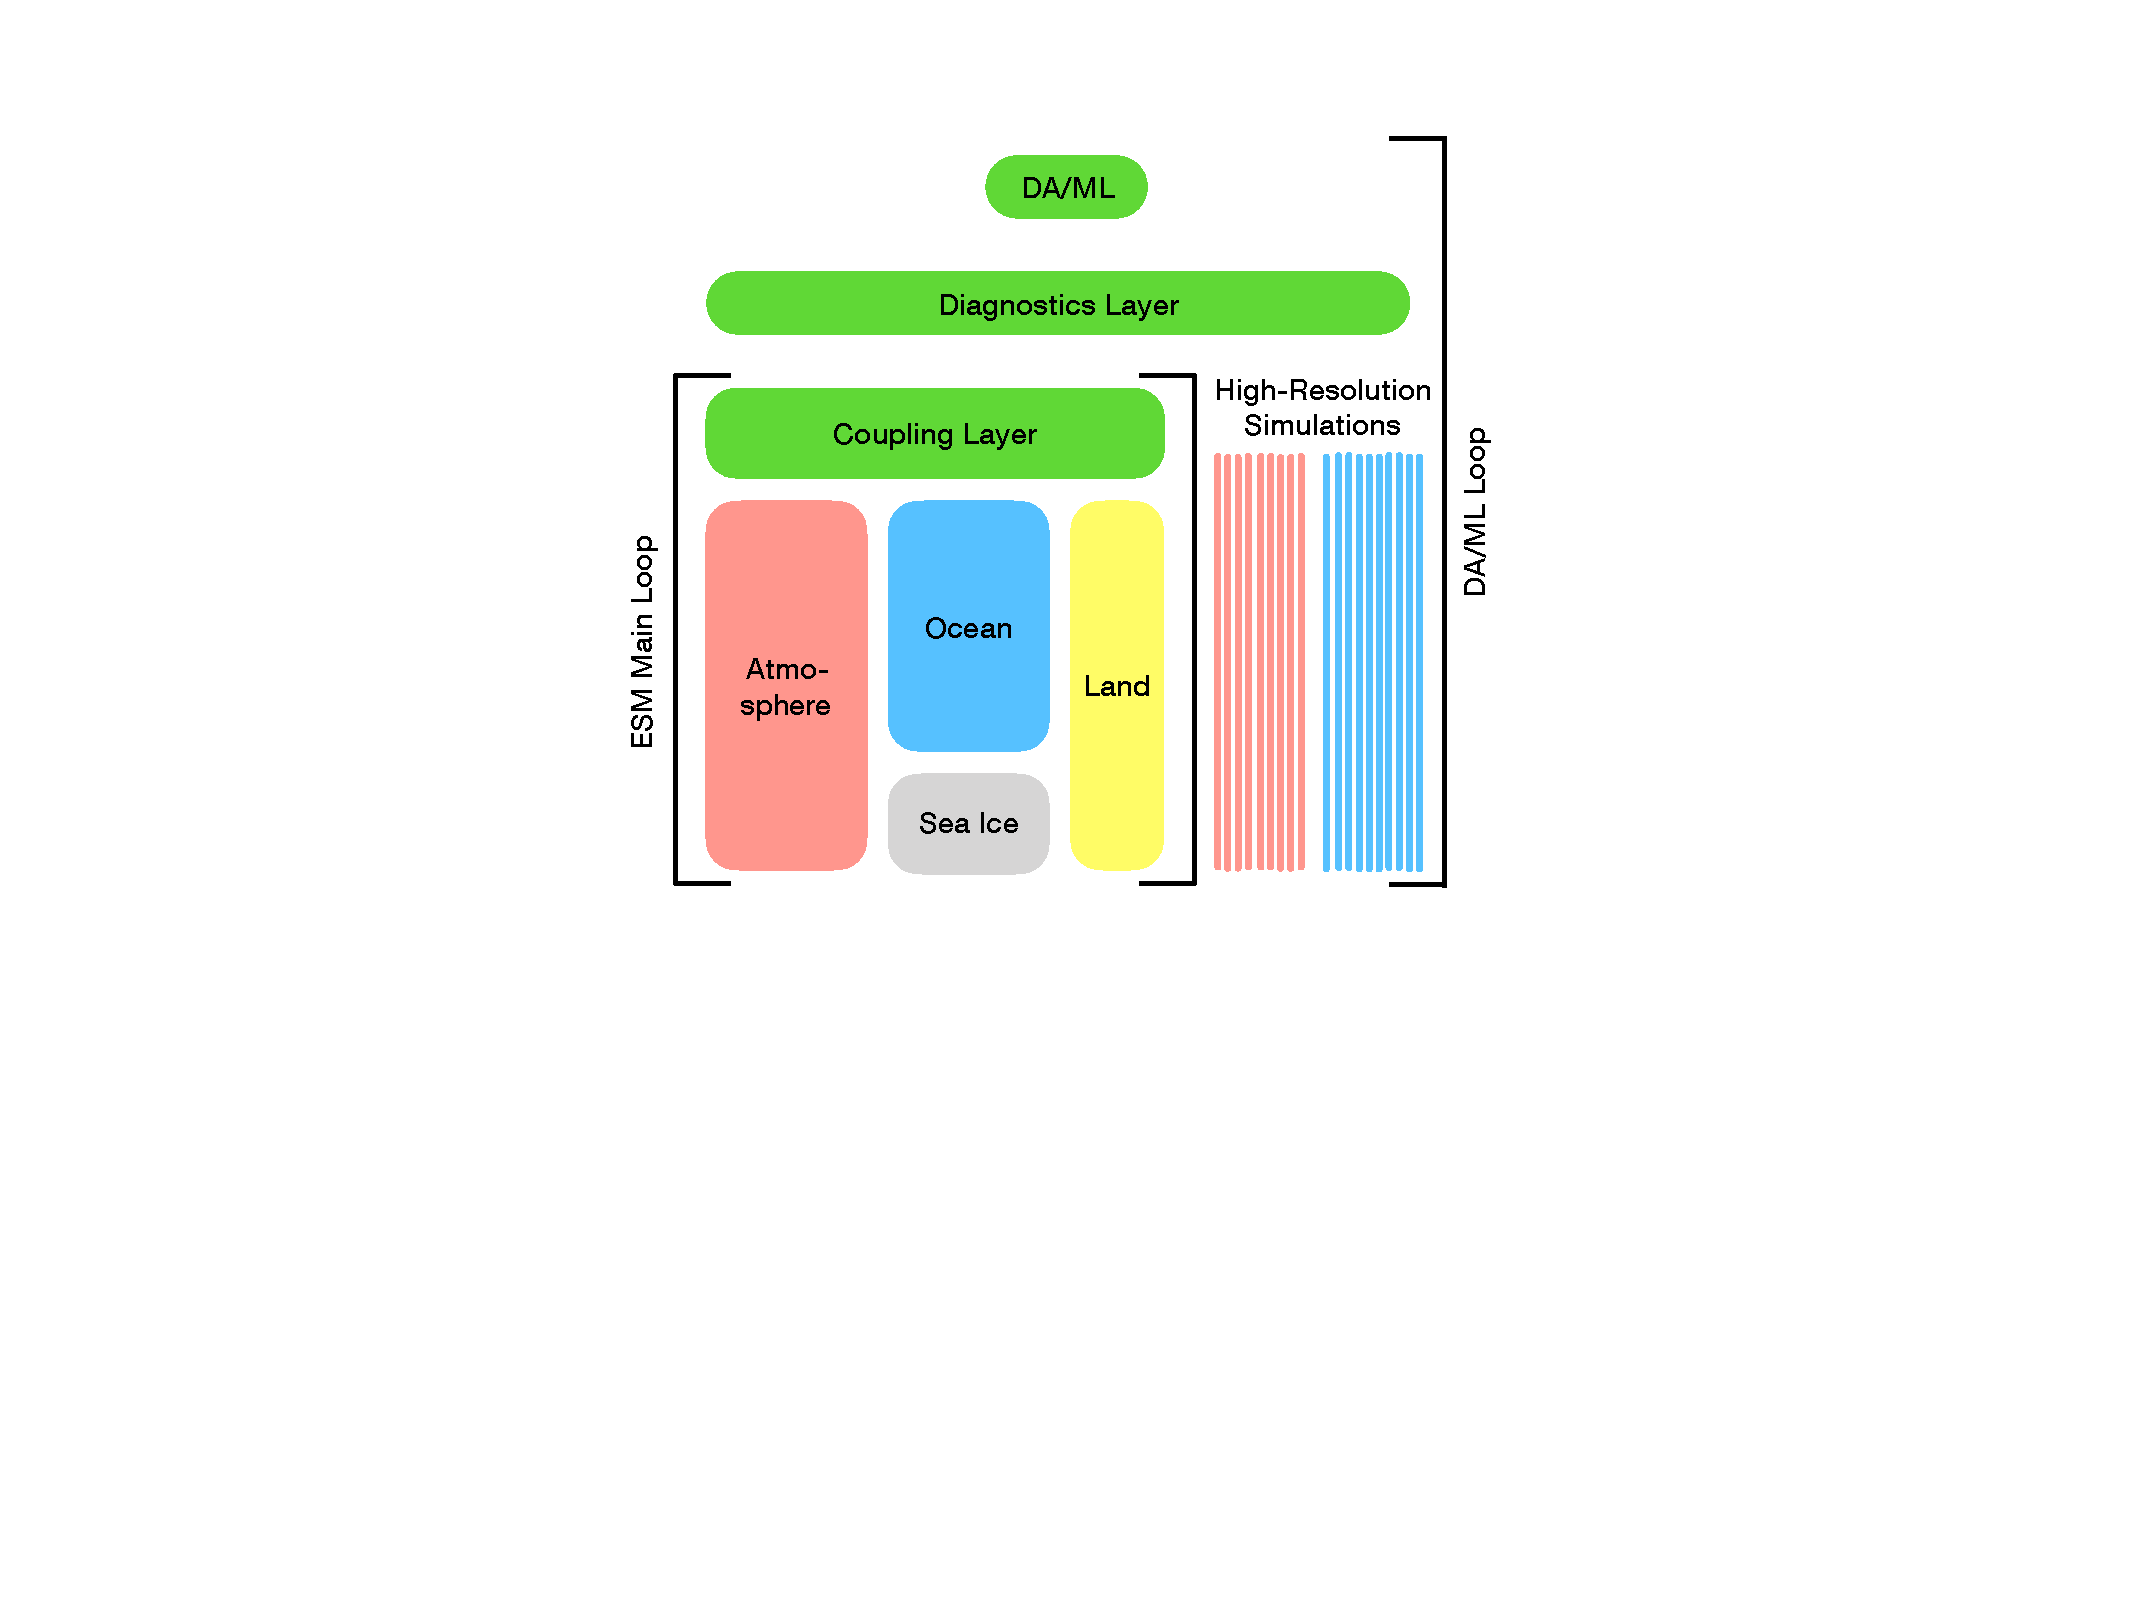
\includegraphics[width=0.65\textwidth]{CLIMA-layers.pdf}}
\caption{\textbf{Schematic of a possible CLIMA computing architecture.} Time increases downward, and processors are indicated across. The different horizontal and vertical extents of the components suggest the degree of parallelism and time of execution (not to scale). The coupling layout with parallel coupling of atmosphere, ocean, and land (component concurrency) and sequential coupling of ocean and sea ice is a possible computational layout; the final layout may be different. Also, other components in addition to those indicated (e.g., a land ice model) may eventually be incorporated into CLIMA.}
\label{f:CLIMA-layers}
\end{figure}

\subsection{Targeted High-Resolution Simulations}

\paragraph{Concepts}
\begin{itemize}
    \item Local high-resolution simulations can provide information about uncertain computable parameters $\vec{\theta}_c$ in SGS processes where observations alone do not provide sufficient information about them. This can include high-resolution simulations of atmospheric clouds, convection, and turbulence, of ocean turbulence both on the mesoscale and submesoscale, and of sea ice dynamics. 
    \item Local high-resolution simulations can also be used to provide detailed climate information where needed, e.g., for local climate impact projection, or as detailed boundary conditions over ice sheets.
    \item Local high-resolution simulations are nested within small areas of the respective ESM component models. For example, atmospheric LES are spun off from the atmosphere model component, nested in small areas (e.g., a grid column) of the global model. Ocean mesoscale-resolving simulations are spun off from the ocean model, in ocean patches that represent a small fraction of the globe, yet are large enough that nonlocal effects (e.g., advection by low-frequency flow components) can be meaningfully represented.
    \item One-way nesting suffices for the high-resolution simulations, which simplifies the embedding of the high-resolution simulations. That is, the global component model drives local high-resolution simulations, but the high-resolution simulations do not feed back onto the global model (except through the information they provide on SGS models). However, even one-way nesting requires the time-evolving large-scale conditions of the host model as drivers and boundary conditions for the high-resolution simulations. 
    \item Conceptually, local high-resolution simulations may be viewed as a time-depen\-dent map $\mathcal{L}$ from ESM state variables $\vec{x}$  to simulated state variables $\vec{\tilde z}$,
    \begin{equation}
    \vec{\tilde z}(t) = \mathcal{L}(\vec{\theta}_n,t; \vec{x}).
    \end{equation}
    The map $\mathcal{L}$ is parameterized by time $t$ and by parameters $\vec{\theta}_n$ that are not computable in the high-resolution simulation and are inherited from the global model (e.g., microphysical parameters in an atmospheric LES). The map $\mathcal{L}$ can depend on the time-history of the state variables $\vec{x}$ up to time $t$, e.g., as time-evolving large-scale drivers and boundary condition for the high-resolution simulation. 
    \item The vector of simulated state variables $\vec{\tilde z}$ contains high-resolution variables aggregated over grid boxes of the global model,  such as the mean cloud cover or liquid water content in a grid box. Their counterparts in the global model are computed by parameterization schemes.
    \item The corresponding variables $\vec{z}$ in the global model are obtained by a time-depen\-dent map $\mathcal{S}$ that takes state variables $\vec{x}$ and parameters $\vec{\theta} = (\vec{\theta}_c, \vec{\theta}_n)$ to $\vec{z}$,
    \begin{equation}
    \vec{z}(t) = \mathcal{S}(\vec{\theta},t; \vec{x}).
    \end{equation}
    The map $\mathcal{S}$ typically represents a single grid column of the ESM with its parameterization schemes, taking as input $\vec{x}$ from the ESM. It is structurally similar to $\mathcal{L}$. Mismatches between $\vec{z}$ and $\vec{\tilde z}$ can be used to learn about computable parameters $\vec{\theta}_c$ because $\vec{\tilde z}$ does not depend on them.
    \item The high-resolution simulated state variables $\vec{\tilde z}$ can also be compared to observations $\vec{\tilde y}$. To do so, a map $\mathcal{Z}$ takes high-resolution simulated state variables to observables,
    \begin{equation}
        \vec{y}(t) = \mathcal{Z}\bigl(\vec{\tilde z}(t)\bigr),
    \end{equation}
    e.g., cloud condensate amounts from LES to observable cloud condensate amounts. Mismatches between observables $\mathcal{Z}(t, \vec{\tilde z})$ and actual observations $\vec{\tilde y}$ can be used to learn about non-computable parameters $\vec{\theta}_n$ because high-resolution simulated state variables $\vec{\tilde z}$ depend on the non-computable parameters, but the observations $\vec{\tilde y}$ do not. 
    \item  Models of non-computable processes in the high-resolution simulation $\mathcal{L}$ and in the single-column model $\mathcal{S}$ need to be represented consistently, so that the non-computable processes in $\mathcal{S}$ are a consistently coarse-grained version of those in $\mathcal{L}$. This is necessary to be able to learn about the computable parameters $\vec{\theta}_c$ without the aliasing errors that would arise if non-computable processes are represented inconsistently across the hierarchy. It is also necessary to be able to use mismatches between $\mathcal{Z}(t, \vec{\tilde z})$ and observations $\vec{\tilde y}$ to learn about non-computable parameters $\vec{\theta}_n$ in the high-resolution model, and use the information so obtained in the ESM. The same code base should be used for non-computable processes in the coarse model and in the high-resolution model. For example, numerical quadrature methods may then be used to coarse-grain the high-resolution process model by sampling from the implied distributions in the coarse model.
\end{itemize}

\paragraph{Goals}
\begin{itemize}
    \item Design the high-resolution simulations to run efficiently on accelerators and in distributed computing environments.  For example, it may be desirable to have one high-resolution simulation per GPU. But more flexible layouts (e.g., one high-resolution simulation spread over several GPUs) should also be possible.
    \item Design the high-resolution simulations to either run concurrently with the global host model (as in Fig.~\ref{f:CLIMA-layers}), with the host model providing time-evolving driving and boundary conditions, or in standalone mode, e.g., with the fixed and/or idealized boundary conditions that are common in atmospheric LES studies. 
    \item Represent non-computable processes in the ESM component models (e.g., microphysics in atmosphere model) and in the high-resolution simulations (e.g., microphysics in atmospheric LES) consistently. That is, the non-computable process models in the ESM need to be consistently coarse-grained version of those in the high-resolution simulations, and the high-resolution simulations need to inherit the non-computable parameters $\vec{\theta}_n$ from the global model.
    \item Target a vertical resolution in atmospheric LES of about 10~m or finer, and a horizontal resolution of 50~m or finer. These are the minimum resolutions necessary to begin to resolve the challenging dynamics of stratocumulus clouds. 
    \item \hl{Ocean}
    \item Make it easily addressable from the DA/ML layer at which physical locations high-resolution simulations are nested in the global model, to be able to target high-resolution simulations where they have the greatest impact on learning of parameters and reducing uncertainties. 
\end{itemize}



\subsection{DA/ML Layer}

\paragraph{Concepts}
\begin{itemize}
    \item The DA/ML layer implements the algorithms for simultaneous learning about parameters (and parameteric functions) $\vec{\theta}$ in all component models, for example, learning about parameters in the atmosphere, ocean, land, ice, and biosphere models at the same time. The DA/ML layer allows for learning about the parameters both from observations and from targeted high-resolution simulations. It sits at the interface of models and data and fuses both. It also targets high-resolution simulations where they have large impact on learning about parameters. 
    \item From the perspective of the DA/ML layer, the ESM is a function $\mathcal{G}$, parameterized by time $t$, that maps parameters $\vec{\theta}$ characterizing uncertain processes to climate state variables $\vec{x}$:
    \begin{equation}
    \vec{x}(t) = \mathcal{G}(\vec{\theta}, t).
    \end{equation}
    The state variables $\vec{x}$ can include temperatures, humidity variables, and cloud, cryosphere, and biogeochemical variables, and the map $\mathcal{G}$ may depend on initial conditions and time-evolving boundary or forcing conditions. The vector of parameters $\vec{\theta}$ can include traditional parameters in SGS models (e.g., entrainment rates in convection parameteriations, turbulent diffusivities etc.), parameters appearing in parametric functions in SGS models about which we want to learn from data (e.g., functions encoding how entrainment rates depend on environmental variables), or parameters characterizing nonparametric functions in SGS models, such as Gaussian process models \citep{Rasmussen06a} included as a flexible representation of error in the explicitly modeled processes.  
    \item The map $\vec{y}(t)=\mathcal{H}\bigl(\vec{x}(t)\bigr)$ takes ESM state variables $\vec{x}$ to observables $\vec{y}$. Because $\vec{y}$ is parameterized by $\vec{\theta}$, while the actual observations $\vec{\tilde y}$ are independent of the parameters $\vec{\theta}$, mismatches $\vec{y} - \vec{\tilde y}$ can be used to learn about the uncertain parameters $\vec{\theta}$. 
    \item Similarly, the map $\vec{z}(t) = \mathcal{S}(\vec{\theta},t; \vec{x})$ (a single-column model) takes state variables $\vec{x}$ to variables $\vec{z}$ that are computable in high-resolution simulations $\mathcal{L}$. Crucially, the map $\mathcal{S}$ generally depends on all parameters $\vec{\theta}=(\vec{\theta}_c, \vec{\theta}_n)$, while $\mathcal{L}$ only depends on non-computable parameters $\vec{\theta}_n$. Thus, mismatches $\vec{z}(t) - \vec{\tilde z}(t)$ can be used to learn about the computable parameters $\vec{\theta}_c$.
    \item Additionally, the map $\vec{y}(t) = \mathcal{Z}\bigl(\vec{\tilde z}(t)\bigr)$ takes high-resolution state variables $\vec{\tilde z}$ to observables $\vec{y}$. Because $\vec{\tilde z}$ is parameterized by non-computable parameters $\vec{\theta}_n$, but $\vec{\tilde y}$ is not, mismatches $\mathcal{Z}\bigl(\vec{\tilde z}(t)\bigr) - \vec{\tilde y}$ can be used to learn about the non-computable parameters $\vec{\theta}_n$.
    \item We generally define objective functions using time-averaged statistics. We denote the time average of a function $\phi(t)$ over the time interval $[t_0,t_0+T]$ by
    \begin{equation}\label{e:Tavg}
    \langle \phi \rangle_T = \frac{1}{T} \int_{t_0}^{t_0+T} \phi(t) \, dt.
    \end{equation}
    (Extensions to data that are not averaged in time, e.g., to assimilate ocean states or data from Argo floats, will be considered as needed.) \hl{Do we need this right away? If so, would someone be willing to take on modifying the text here?}
    \item The observational objective function can then be written in the generic form
    \begin{equation}\label{e:obj_o}
    J_o(\vec{\theta})=\frac{1}{2}\| \langle \vec{f}(\vec{y})  \rangle_T - \langle \vec{f}(\vec{\tilde y})
    \rangle_T \|_{\Sigma_y}^2
    \end{equation}
    with the 2-norm
    \begin{equation}
    \|\cdot\|_{\Sigma_y}=\|\Sigma_y^{-1/2}\cdot\|
    \end{equation}
    normalized by error standard deviations and covariance information captured in $\Sigma_y$. The choice of variance/covariances will have a significant impact on the effectiveness of the learning, as it assigns relative weights to different sources of data. The relevant components of $\Sigma_y$ may be chosen very small for quantities that are used as constraints on the ESM (e.g., the requirement of a closed global energy balance at TOA).
    \item The function $\vec{f}$ of the observables typically involves first- and second-order quantities, for example,
    \begin{equation}
    \vec{f}(\vec{y}) = \left( 
    \begin{array}{c} 
    \vec{y}\\
    y_i' y_j'
    \end{array}
    \right),
    \label{e:of}
    \end{equation}
    where, for any observable $\phi$, $\phi'(t) = \phi(t) - \langle \phi \rangle_T$ denotes the fluctuation of $\phi$ about its mean $\langle \phi \rangle_T$. With $\vec{f}$ given by \eqref{e:of}, the objective function penalizes mismatch between the vectors of mean values $\langle \vec{y} \rangle_T$ and $\langle \vec{\tilde y}\rangle_T$ and between the covariance components $\langle y_i' y_j' \rangle_T$ and  $\langle \tilde y_i' \tilde y_j' \rangle_T$ for some indices $i$ and $j$. However, $\vec{f}$ may also include higher-order statistics, such as high percentiles of the precipitation distribution, to penalize mismatches between simulated and observed statistics of precipitation extremes. 
    \item Similarly, for the mismatch between the ESM and high-resolution simulations, we define an objective function analogously to that for the observations through
    \begin{equation}\label{e:obj_hr}
    J_s(\vec{\theta}_c)=\frac12\| \langle \vec{g}(\vec{z})  \rangle_T - \langle \vec{g}(\vec{\tilde z})
    \rangle_T \|_{\Sigma_z}^2.
    \end{equation}
    Like the function $\vec{f}$ above, the function $\vec{g}$  typically involves first- and second-order quantities, and $\Sigma_z$ encodes error variances and covariances. (This assumes that high-resolution simulations in any location are run over the same interval $[t_0, t_0+T]$ over which ESM statistics are accumulated. This is how we will implement the learning algorithms for now. The assumption may be relaxed later.) 
    \item An objective function $J_z(\vec{\theta}_n)$ for the mismatch between high-resolution simulations  $\mathcal{Z}(t, \vec{\tilde z})$ and observations $\vec{\tilde y}$ is defined analogously. 
    \item Learning about parameters $\vec{\theta} = (\vec{\theta}_c, \vec{\theta}_n)$ in CLIMA proceeds through minimizing $J_o(\vec{\theta})$, $J_s(\vec{\theta_c})$, and $J_z(\vec{\theta_n})$. We will have to determine how to formalize the interaction between the different objective functions in this multi-objective optimization problem.
\end{itemize}

\paragraph{Goals}

\begin{itemize}
    \item Design the DA/ML layer to be as general purpose as possible, so that its algorithms can also be used for statistical learning problems in other sciences.
    \item Use gradient-free optimization algorithms (to avoid the stasis in model development that often arises when manually manipulated ajoints are required).
    \item Develop, test, and implement algorithms for optimizing parameters $\vec{\theta}$ that require as few ESM runs as possible---$O(1000)$ ESM runs, with embedded high-resolution simulations, over timescales of seasons are feasible. 
    \item Develop, test, and implement algorithms for quantifying uncertainties about parameters $\vec{\theta}$, via emulation of the functions $\vec{f}$, $\vec{g}$ etc. \citep{Kennedy01a,OHagan06a}.
\end{itemize}

\subsection{Diagnostics Layer}

\paragraph{Concepts}

\begin{itemize}
    \item  Given observations and model output, both from the global model and high-resolution simulations, the diagnostics layer computes the statistics of model variables and observations that the DA/ML layer requires.
    \item Specifically, the diagnostics layer needs to provide the functions $\vec{f}$, $\vec{g}$ etc. and time averages $\langle \cdot \rangle_T$. These functions should be usable with input data from observations $\vec{\tilde y}$, global model state variables $\vec{x}$, high-resolution state variables $\vec{\tilde z}$, and single-column model variables $\vec{z}$.
    \item Because I/O can be slow and may generate unwieldy amounts of data, the diagnostics layer should be able to accumulate the statistics the DA/ML layer needs from the ESM and from the targeted high-resolution simulations on the fly, without intermediate write-outs to disk.
\end{itemize}

\paragraph{Goals}

\begin{itemize}
    \item Design and implement a diagnostics layer that can accumulate statistics from global host models, targeted high-resolution simulations, and observations. Which statistics to accumulate should be easily addressable from the DA/ML layer.
    \item Design and implement a broad-purpose API for the diagnostics layer, so it can be used with diverse sources of input data. 
    \item Provide a (possibly web-based) graphical user interface that allows users to easily examine output from the various models and compare it with observations.
\end{itemize}

\subsection{Coupling Layer}

\paragraph{Concepts}

\begin{itemize}
    \item The coupling layer lies at the interface between the DA/ML and diagnostics layers, on the one hand, and the component models, on the other hand (Fig.~\ref{f:CLIMA-layers}). It coordinates the exchange of data between component models such as the atmosphere, land, and ocean models.  
    \item The coupling layer needs to allow for conservative exchange of data (e.g., surface stresses, energy fluxes) across the component models' grids. To facilitate this exchange, it will be helpful to co-align grid nodes across the component models to the extent possible (e.g., atmosphere and ocean, and atmosphere and land, should share some nodes, even if they have different resolutions).
    \item Making internal data structures consistent across the component models will facilitate design of the coupling layer. 
    \item The coupling layer needs to accommodate the parallel computing layout of the model components and needs to allow parallel data exchange between the model components \citep[e.g.,][]{Larson05a}. It may be desirable to run model components concurrently in parallel \citep{Balaji16a}, e.g., running the atmosphere model in parallel with the ocean model (as in Fig.~\ref{f:CLIMA-layers}). However, numerical coupling instabilities can arise when doing so \citep{Hallberg14a}. The timestepping strategy of the coupling needs to be chosen to guarantee stable coupling. 
\end{itemize}

\paragraph{Goals}

\begin{itemize}
    \item Devise a stable time-stepping strategy for the component coupling.
    \item Design and implement a parallel coupling layer with conservative exchanges of mass, water, momentum, and tracers across model components.  
\end{itemize}

\subsection{Component Models}

The component models at the center of the ESM should function in a coupled configuration, and learning about parameters in them should occur simultaneously, to ameliorate problems arising from correlated errors among model components. Yet each model component should also be able to function as a standalone executable. The component models should share as much code (e.g., fluid dynamics operators, compute kernels) and inputs (e.g., topography/bathymetry databases) as possible, to avoid unnecessary growth of the total code base and make adaptation of the code to different planetary configurations as easy as possible.

\subsubsection{Atmosphere Model (CLIMA-atmos)}

\paragraph{Concepts}

\begin{itemize}
    \item The atmosphere model provides approximate solutions to the equations of fluid mechanics and thermodynamics on a rotating sphere. It consists of a dynamical core and parameterizations. The dynamical core discretizes the 3D compressible Euler equations and thermodynamic equations on a sphere. Parameterizations are needed principally for radiative transfer and for dynamical process at scales below the resolution of the global grid, such as SGS turbulence, convection, cloud microphysics, and gravity waves.
    \item Large-eddy simulations provide approximate solutions to the same (non-hydrostatic) equations as the atmosphere dynamical core, just at higher resolution and, because of the large computational expense, in limited domains. LES resolutions needed to resolve the dynamics of cumulus clouds are in the range of $O(100~\mathrm{m})$. To resolve the dynamics of stratocumulus clouds under a sharp inversion (a nearly discontinuous thermodynamic interface common in the subtropics), LES require resolutions of at least 50~m in the horizontal and 10~m in the vertical. Avoiding spurious mixing in the numerical solution of the equations of motion (caused, e.g., by spuriously oscillatory numerics interacting with dissipative SGS schemes) is essential for faithful simulations of the climatically important stratocumulus clouds \citep{Pressel17a}.
    \item The atmosphere dynamical core needs to be able to run at resolutions ranging from hundreds of kilometers in the horizontal (for prototyping and testing) to kilometers (where deep convection begins to be resolved).
    \item Scalability of the atmosphere model on a variety of hardware architectures, including accelerators, is paramount. This may require redesigning existing parameterizations, e.g., for radiative transfer, which currently involve extensive nonlocal operations (vertical integrals). 
    \item For historical reasons, distinct parameterizations have been employed for processes lying on a continuous spectrum, such as boundary-layer turbulence, shallow (non-precipitating) convection, and deep (precipitating) convection. Parameterizations for processes such as microphysics (e.g., rain droplet formation) and radiative transfer typically have not strongly interacted with parameterizations for dynamical processes, although in nature the processes do strongly interact. This has led to correlated and compensating errors between the parameterization schemes; it leads to identifiability problems in a DA/ML approach to parameterizations. For our DA/ML approaches, it will be important to devise process-informed parameterization schemes that represent processes that lie on a continuous spectrum in a unified manner, with as few parameters as possible. Parameterizations also need to be able to adapt to different host model resolutions (be ``scale aware'') and to refine themselves as more data informing the processes become available. Error models (e.g., Gaussian processes) may also be incorporated directly in parameterization schemes and be estimated along with parameters and parametric functions in the parameterization schemes. 
    \item Parameterizations should be developed in the form of continuous differential equations, which can then be discretized consistently with the host model (use the same compute kernels). However, parameterizations may employ resolutions and time steps that differ from those in the host model. 
    \item It would be desirable for the global atmosphere model, parameterizations, and LES to share the same prognostic variables. This means that using moist conserved variables (e.g., liquid-ice static energies) throughout may be advantageous. Variables that are nonlinear functions of temperature (e.g., entropies) should be avoided, because they make it computationally expensive to retrieve temperature.
\end{itemize}

\paragraph{Goals}

\begin{itemize}
    \item Develop an atmosphere dynamical core that employs state-of-the art numerics, can exploit emerging computing architectures, and can run embedded high-resolution simulations (LES) on the fly.
    \item Develop atmosphere parameterizations suitable for DA/ML approaches, first focusing on turbulence, convection, and clouds, and then expanding to gravity waves and (if needed) radiative transfer.
    \item Demonstrate automated learning about parameterization schemes from observational data and high-resolution simulations nested in the atmosphere model.
\end{itemize}

\subsubsection{Ocean Model (CLIMA-ocean)}

\subsubsection{Land Model (CLIMA-land)}

\paragraph{Concepts}

\begin{itemize}
    \item Land models consists of models for the hydrology of ground and surface water (especially river runoff) and for the land biosphere. These two types of models interact closely but should be treated distinctly because we know the equations for modeling the physics of water flow, and can coarse grain and approximate the equations systematically. However, the biosphere must be modeled more empirically. 
\end{itemize}

\subsection{Compute Kernels}

\subsection{Parallel Communications/Services}

\section{General Guidelines}

\begin{itemize}
    \item Implement best practices for scientific computing \citep[e.g.,][]{Wilson14a}, including
        \begin{enumerate}
            \item Make names consistent, distinctive, and meaningful. For variable names, follow CMIP conventions where possible and practicable (http://clipc-services.ceda.ac.uk/dreq/index.html).
            \item Use a build tool to automate workflows.
            \item Make incremental changes, with version control (GitHub).
            \item Modularize code rather than copying and pasting (DRY--don't repeat yourself).
            \item Integrate continuously and employ unit testing (try to develop tests before developing the code, and focus on short unit tests, which give more valuable information when they fail; make unit tests meaningful, e.g., check for conservation of properties that should be conserved).
            \item Make code correct first and fast second (then use profilers to identify bottlenecks).
            \item Document design and purpose (document interfaces and embed documentation in code).
            \item Collaborate (pre-merge code reviews, pair programming to bring new people up to speed, for tricky problems; use issue tracking on GitHub).
            \item Design APIs for the simplest cases first, add options for more flexible use.
            \item Shared code ownership is the goal; siloed knowledge is bad.
        \end{enumerate}
    \item Limit external package dependency as much as possible to facilitate portability. Where package dependencies are essential, use common packages with a broad user base (e.g., MPI, NetCDF library)
    \item Collect all input parameters (physical constants, topography/bathymetry datasets etc.) in one central place, where they are easy to modify and are shared by all components of the code. Input parameters should not be multiply defined for different code components.
    \item \hl{[Add and expand!]}
\end{itemize}

\section{Objectives and Key Results for Years 1--3}

We will pursue several key objectives in years 1--3 (by 2021), and we will measure progress by achievement of the key results listed for each objective.
\begin{enumerate}
    \item \textbf{Develop scalable atmosphere and ocean dynamical cores that exploit emerging computing architectures and can run high-resolution simulations on the fly.}
    \begin{enumerate}
        \item Demonstrated scaling of atmosphere and ocean models on CPUs and GPUs \hl{[can we say something more precise and quantitatively measurable here?]}.
        \item Demonstration of at least 100 concurrent high-resolution simulations (LES) running alongside global atmosphere model.
        \item \hl{Something specific and measurable about the ocean and high-resolution simulations}
    \end{enumerate}
    
    \item \textbf{Develop atmosphere and ocean process models suitable for DA/ML approaches.}
    \begin{enumerate}
        \item Demonstrate scale-adaptive parameterization schemes for atmospheric turbulence, convection, and clouds (including microphysics) that can learn from observations and LES.
        \item Show that the atmospheric parameterization schemes adequately capture cloud and boundary layer regimes such as stable polar boundary layers, stratocumulus-topped boundary layers, shallow cumulus convection, and deep convection.
        \item Demonstrate a gravity-wave parameterization that can learn from observations.
        \item \hl{Ocean process models?}
        
    \end{enumerate}
    
    \item \textbf{Develop fast and efficient DA/ML algorithms.}
     \begin{enumerate}
        \item \hl{Something specific and quantitative here: e.g., optimization with about 1000 ESM runs, UQ targets etc.}
    \end{enumerate}
    
    \begin{figure}[htb]
     \centerline{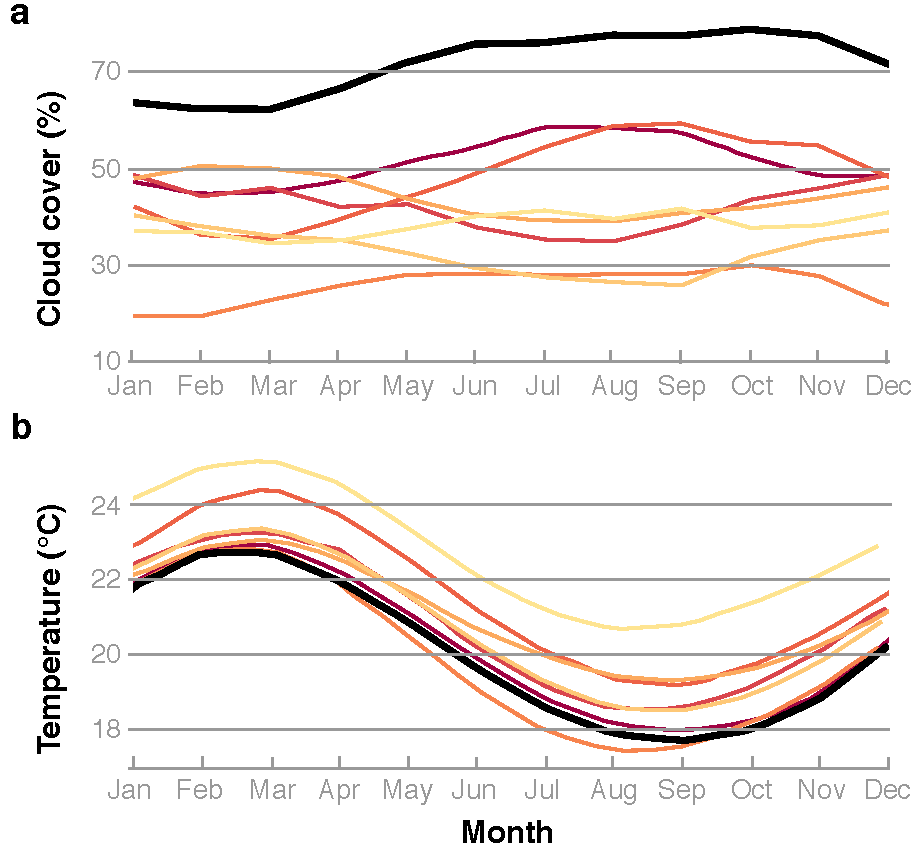
\includegraphics[width=.6\textwidth]{Lin-Sc-bias.pdf}}
      \caption{\textbf{Cloud cover bias in current climate models.} Annual cycle of (a) cloud cover and (b) sea surface temperature off the coast of subtropical South America from observations (black) and in current climate models (colors). Data from \protect\citet{Lin14b}.}\label{f:Sc-bias}
    \end{figure}
    \item \textbf{Demonstrate atmosphere and ocean models and learning from observational data (primarily reanalysis) and nested high-resolution simulations.}
    \begin{enumerate}
        \item Demonstrate atmosphere-only simulations that learn automatically from observations and nested high-resolution simulations, in two configurations: (i) driven by observed sea surface temperatures, and (ii) coupled to a slab ocean with observed ocean energy fluxes. (Configuration (ii) will clearly expose biases in the surface energy balance resulting, e.g., from biases in cloud cover.)
        \item Demonstrate a substantial reduction is biases relative to current (CMIP5) simulations: (i) reduce tropical low-cloud cover biases to less than 10\% (compare Fig.~\ref{f:Sc-bias} for current model biases) (ii) reduce polar temperature biases to less than 2~K and sea ice cover biases to less than $2\times 10^6~\mathrm{km^2}$ (compare Fig.~\ref{f:polar-bias} for current model biases); (iii) reduce global-mean precipitation biases by a factor 2.
        \item \hl{ocean targets? ML depth?}
    \end{enumerate}
    \begin{figure}[htb]
      \centerline{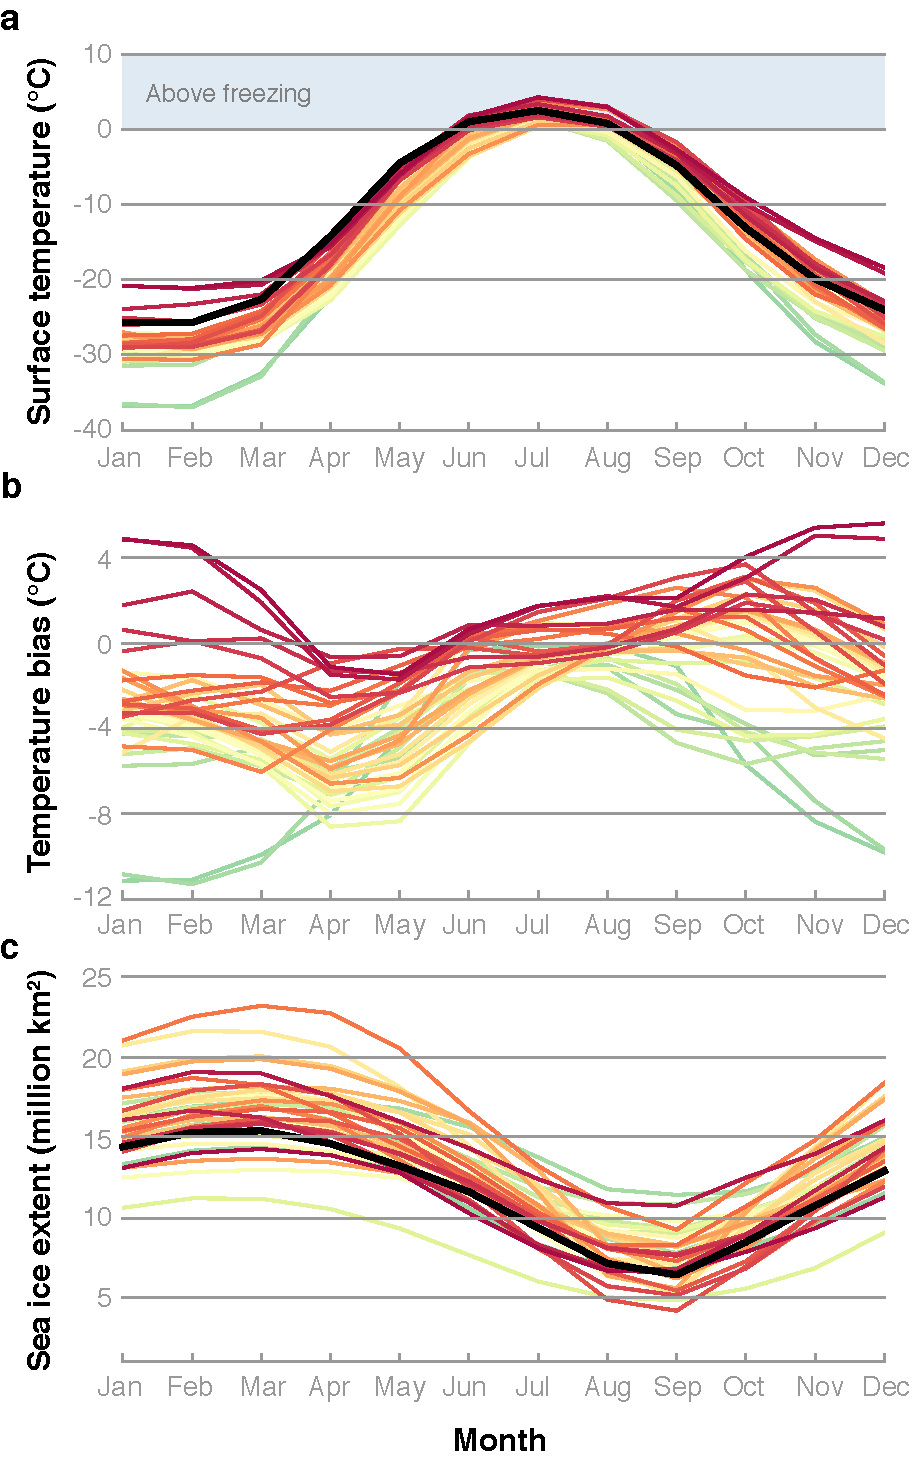
\includegraphics[width=.6\textwidth]{CMIP5-Arctic}}
       \caption{\textbf{Annual cycle of observed and simulated Arctic temperatures and sea ice extent.}; (a) Surface temperature (65$^\circ$--90$^\circ$N), (b) surface temperature bias (difference between simulations minus observations), and (c) sea ice extent from satellite observations (black) and in climate models (colors).}\label{f:polar-bias}
    \end{figure}
    
    \item \textbf{Proof-of-concept of uncertainty quantification in process models and climate predictions.}
    \begin{enumerate}
        \item Demonstrate accuracy of UQ in perfect-model settings in idealized (e.g., aquaplanet) contexts, where accurate UQ with MCMC is still feasible. 
        \item Demonstrate UQ in atmosphere-only models (driven by observed SST, or coupled to slab ocean).
        \item Demonstrate global UQ in climate predictions through ensemble of simulations drawn from posterior density of parameters in process models.
        \item Demonstrate local climate predictions with ensemble of targeted high-resolution simulations, with parameters drawn from posterior in process models.
        \item \hl{oceans?}
    \end{enumerate}
\end{enumerate}
The key results listed are intentionally ambitious. Some may be a stretch to achieve. We can consider ourselves successful if we achieve about 70\% of the key results. 

\clearpage
\bibliographystyle{agufull08}
\bibliography{CLIMA-refs}

\end{document}
